% Define a custom style for JSON formatting
\lstdefinelanguage{json}{
    basicstyle=\ttfamily\small,
    numbers=left,
    numberstyle=\tiny\color{gray},
    stepnumber=1,
    numbersep=8pt,
    showstringspaces=false,
    breaklines=true,
    frame=single,
    backgroundcolor=\color{gray!10},
    keywordstyle=\color{blue},
    stringstyle=\color{red},
    morestring=[b]",
    morecomment=[l]{:}
}




\chapter{System Architecture}

This section presents the general architectures of the systems we used for the development and experiments in our system. We illustrate the Extraction, Transformation, and Load (ETL) pipeline we used for the misinformation rebuttal. Additionally, we have our misinformation classification process, where we classify the health misinformation and refute it. Finally, we have the UI design where users interact with the texts and the results. 

\section{Research Paper ETL Pipeline}

Our model must use credible sources of information to rebut misinformation. We identified PubMed \cite{pubmed}, an online library that contains peer-reviewed medical literature. We want to extract the papers and store them in a vector database. To extract these papers, we used the BioC API \cite{bioinformatics}, which has access to the PubMed library. However, the API needs the research paper's identifier, known as PubMed Central (PMC) ID. We design a scraper to extract these identifiers from the official PubMed site. The pipeline in Figure \ref{fig:etl} shows the processes of data extraction. 

\begin{figure}[H]
	\begin{center}
		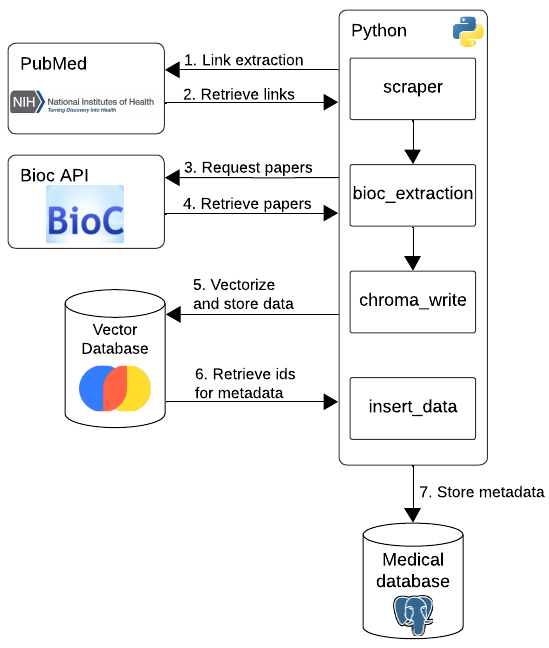
\includegraphics[width=0.75\textwidth]{images/ETL_Pipeline.png} %specify width
	\end{center}
	\caption{Medical Data Extraction Pipeline} %specify caption
	\label{fig:etl}
\end{figure}

\subsection{Scraper}
The first step of the pipeline was identifying what papers we needed to extract. We selected 17 topics for the data extraction process, that can be seen in Table \ref{table:topics}.

\begin{table}[!ht]
	\centering
	\caption{Topics for Research Paper Extraction}
	\begin{tabular}{||c | c||} 
			\hline
			 \multicolumn{2}{||c||}{\textbf{Topics}} \\ [1.5ex] 
			\hline
			allergy  & covid vaccine \\ [1ex]
			\hline
			bird flu & flu vaccine \\ [1ex]
			\hline
			cancer & headache \\ [1ex]
			\hline
			chickenpox & influenza\\ [1ex]
			\hline
			common cold & monkeypox \\ [1ex]
			\hline
			conjunctivitis & stomach aches \\ [1ex]
			\hline
			covid sickness & swine flu \\ [1ex]
			\hline
			covid symptoms & zika\\ [1ex]
			\hline
			covid treatment &  \\ [1ex]
			\hline
			\end{tabular}
	\label{table:topics}
\end{table}


To extract them, we built a scraper in Python using Selenium and BeautifulSoup libraries. We used Selenium to retrieve the web source from PubMed's website, and BeautifulSoup was used to get the links to each paper. These links contained the PMC identifier. For each topic, we selected 5,000 PMC identifiers. These identifiers were grouped by topic and stored locally in Comma Separated Value (CSV) files.

\subsection{BioC API}
After retrieving those identifiers, we need to extract the research papers. Using the PubMed API, BioC, we made requests that returned the documents as JSON. These JSONs were preprocessed to extract texts, and we removed tables and figures. Later, the paper's sections -introduction, methodology, results, and others- were combined as one attribute, excluding references. We removed tables, figures, and references from the context to ensure the chunking process worked appropriately. If the data is not preprocessed, when performing RAG, we can retrieve data that is not useful. After that, we turned the result into a new JSON that contained the research metadata and its context. 

\subsection{Vectorizing data}
After retrieving the data, we need to vectorize the papers. Figure \ref{fig:vector} shows the process of the papers vectorization. First, each research paper’s context was split into chunks using LangChain. Then, we used an LLM, BAAI \cite{bge_embedding}, to embed these chunks. A universal unique identifier (UUID) was combined with each chunk and stored in a Chroma \cite{chroma} database. After uploading the data to Chroma, we added these UUIDs to their JSON. 

\begin{figure}[H]
	\begin{center}
		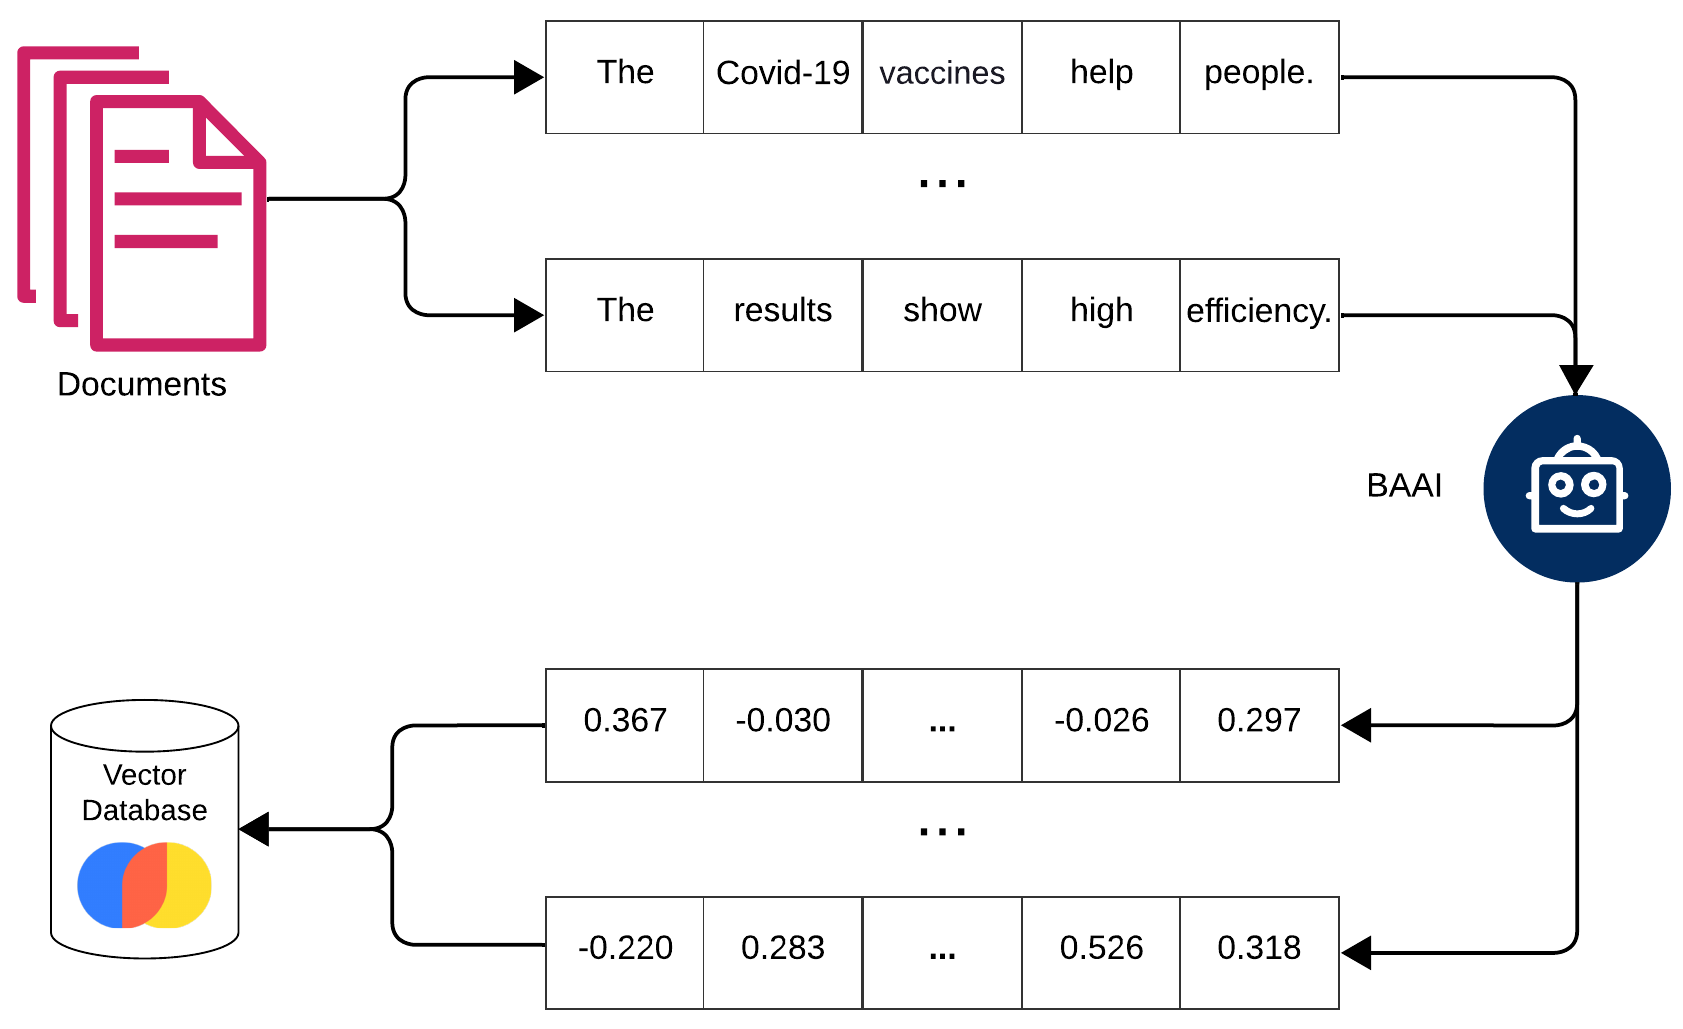
\includegraphics[width=0.9\textwidth]{images/Data_vectorization.png} %specify width
	\end{center}
	\caption{Data Vectorization Process} %specify caption
	\label{fig:vector}
\end{figure}


\subsection{Store metadata}
Now, with all papers vectorized, we upload the metadata into a Postgres database. First, we validate that there are no duplicate records in the system. To prevent duplicates, we search for the paper's reference. If any is found, we delete the chunks from the vector database. Additionally, any research that did not contain at least an abstract was removed. That ensures that there is no repetition or inconsistency when doing the rebuttal. Later, we upload this data into the system following the schema found in Figure \ref{fig:table}. The tables in this schema are as follow:

\begin{description}
	\item{\textbf{Research:}}  The table contains the research paper data. Its attributes are title, which is the research paper title; context, the paper’s text; paper\_ref, the complete reference of the paper, used to prevent duplicates; and fullpaper, which is a boolean that is true if the paper contains an abstract, introduction, methodology, discussion, conclusion, and references.
	\item{\textbf{Chunks:}} This table pairs the UUIDs from the paper's chunks and their respective research record.  
	\item{\textbf{Keyword:}} Some research papers contain keywords that allow the reader to know the subjects mentioned in the paper. 
	\item{\textbf{Author:}} Stores the first and last names of all authors identified in the research paper. 
	\item{\textbf{Reference:}} All references that are present in the research paper.
	\item{\textbf{Topic:}} This contains the different topics used to search the papers.

\end{description}

\begin{figure}[H]
	\begin{center}
		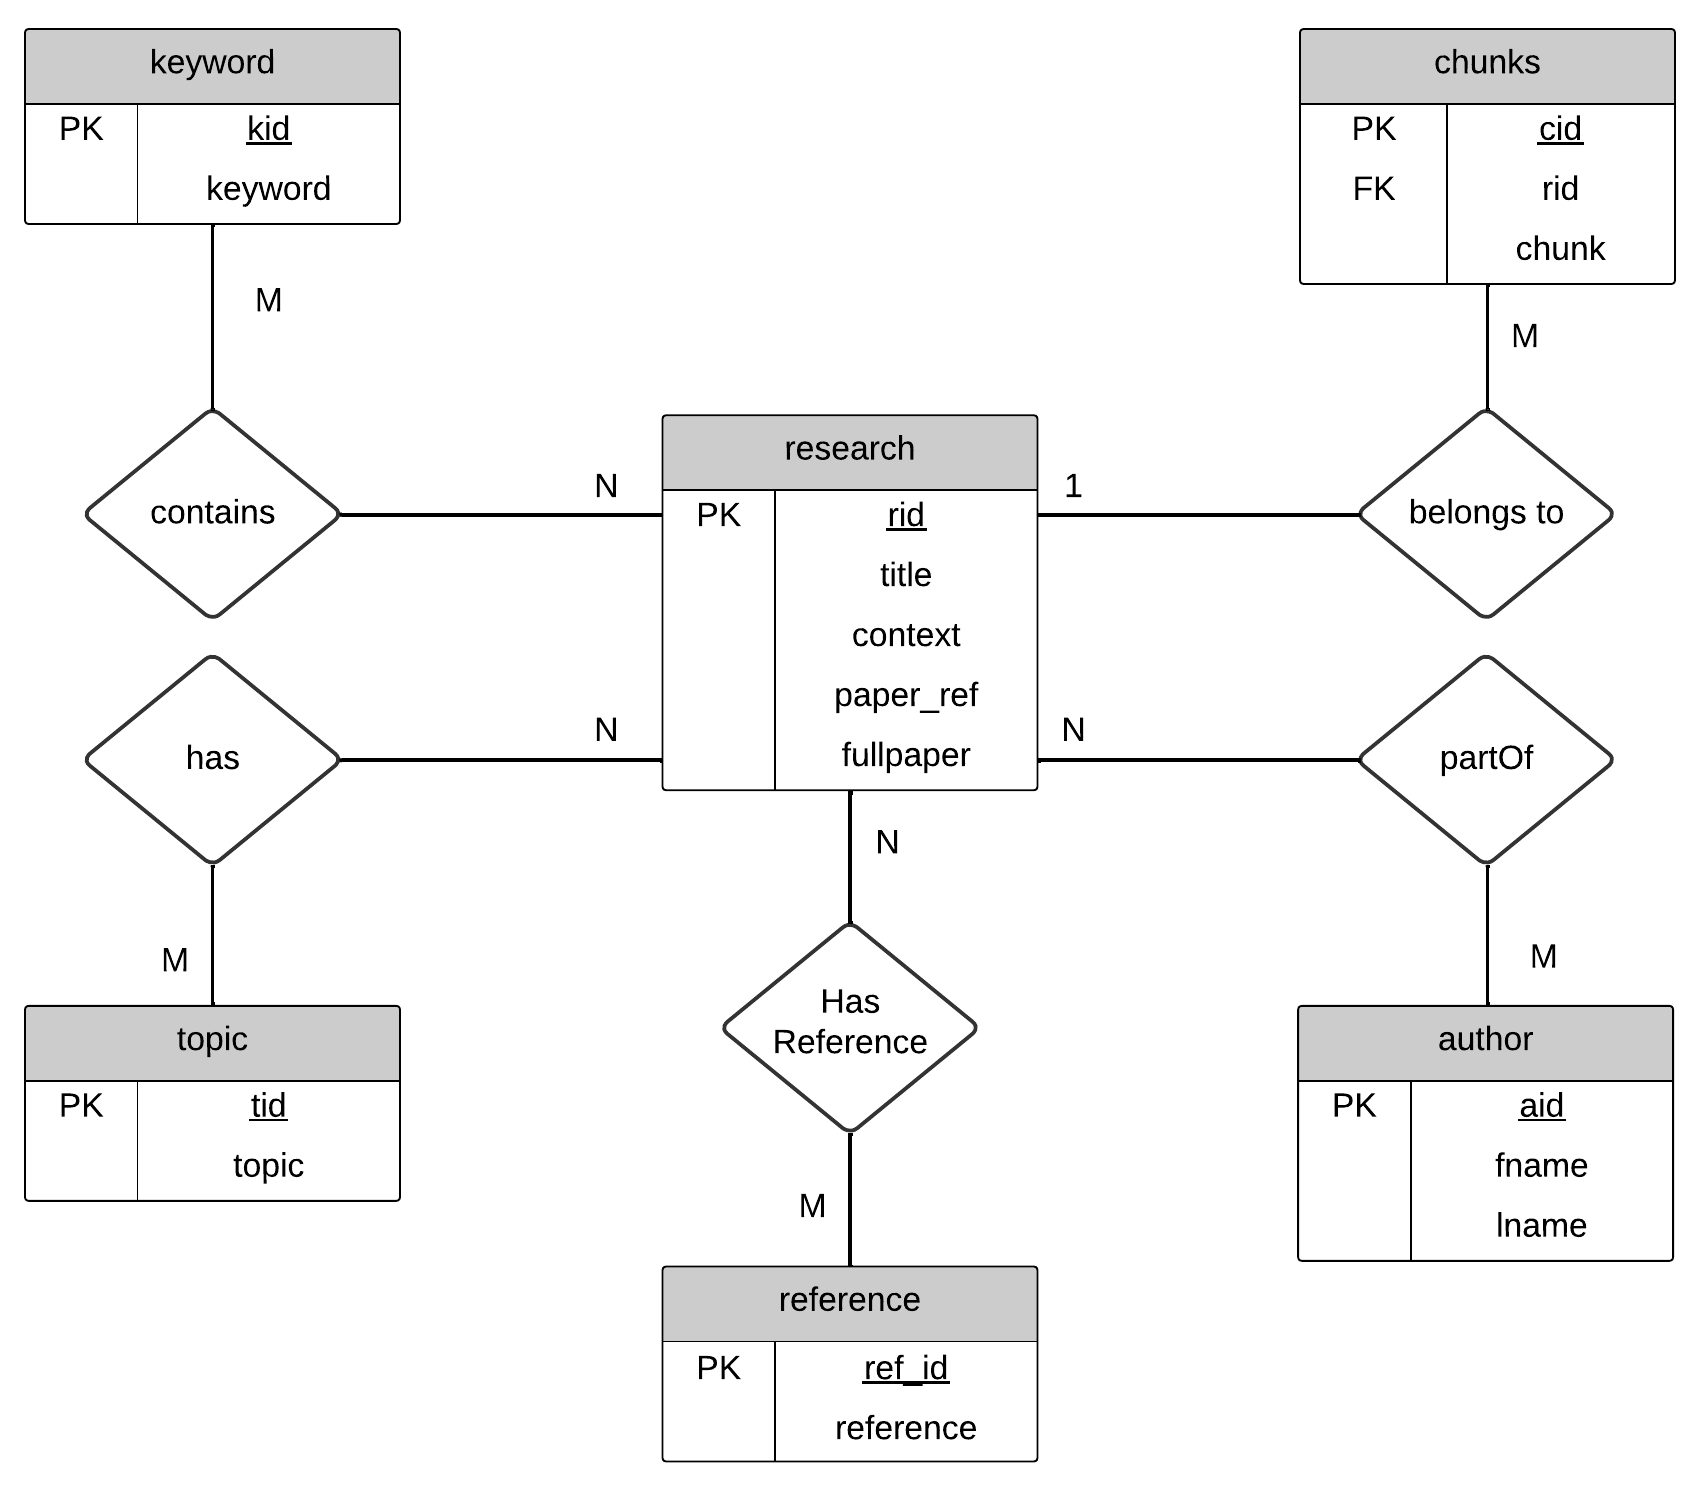
\includegraphics[width=0.9\textwidth]{images/Table_diagram.png} %specify width
	\end{center}
	\caption{Research Papers Schema Diagram} %specify caption
	\label{fig:table}
\end{figure}


We started the search with 85,000 peer-reviewed papers. After finishing the filtering and data cleaning, we ended with 56,365 different research papers. 



\section{Misinformation Rebuttal Pipeline}
After training the models and storing the context for the rebuttal, we create the model pipeline. The pipeline shown in Figure \ref{fig:llm} shows the process of receiving a text, making the classifications, and returning an explanation of why it is misinformation.

\begin{figure}[H]
	\begin{center}
		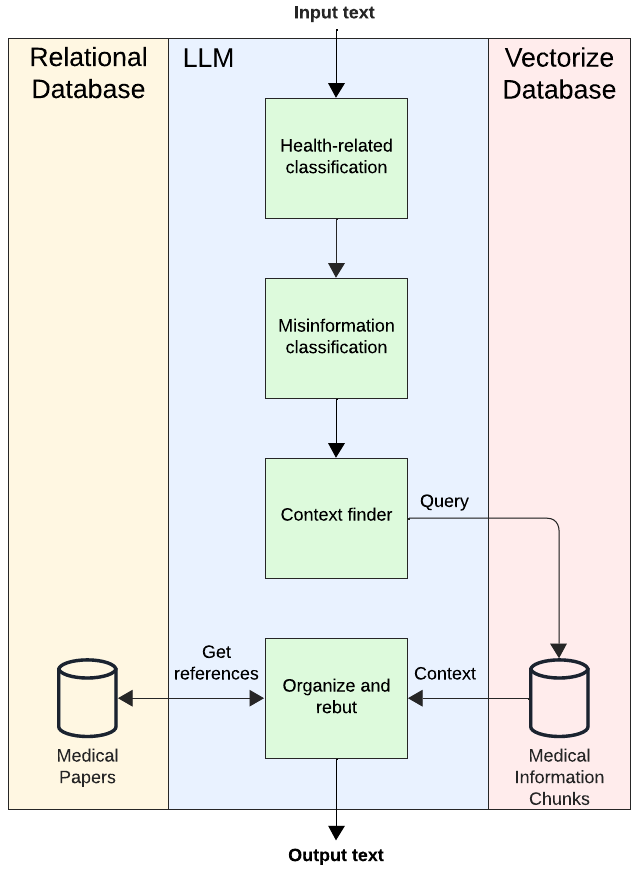
\includegraphics[width=0.75\textwidth]{images/LLM_Pipeline} %specify width
	\end{center}
	\caption{Misinformation Rebuttal LLM System Architecture} %specify caption
	\label{fig:llm}
\end{figure}


\subsection{Health-related Classification}
The first part of the pipeline is determining if the text is related to health. When the system receives the input text, it sends it to a model fine-tuned to classify health-related texts. This model determines whether the input is related, unrelated, or ambiguous.
If the text is health-related, we continue to the next part of the pipeline. When the text is non-related or ambiguous, we end the process. We end this because the topics are out of the model's scope. 

\subsection{Misinformation Classification}
After confirming that the text is health-related, we want to validate that it contains misinformation. The fine-tuned model can only return two possible results: misinformation or non-misinformation. If the model finds no misinformation after evaluating the text,
the final output will return that classification. When the result contains misinformation, we start the search for research papers that be used to rebut the message.

\subsection{Context Finder}
Before starting the search on the vector database, we must understand the topic of the text. To automate this process and generate a query as precise as possible, we use Ollama \cite{ollama}. That tool allows us to execute locally a pre-trained LLM that generates text. Thus, we send a query to Ollama asking it to make a one-sentence query for the vector database related to the input.

 
 \begin{tcolorbox}[colback=gray!10, colframe=black!70, title=Input]
\texttt{%
\#nih fauci, @cdcdirector @sgottliebfda \&amp; @barda bright expected to be grilled tomorrow over ineffective \#flu vaccine at @housecommerce \#suboversight bets on fauci saying universal \#influenza vax in 5, maybe 10 years? my preview here: \url{https://t.co/fsqefwhik7} \#cdc \#fda \#vaccines%
}
\end{tcolorbox}

\begin{tcolorbox}[colback=white, colframe=black!70, title=Output]
\textit{%
Flu vaccine effectiveness and future universal influenza vaccination strategies.%
}
\end{tcolorbox}
 
The above example shows that Ollama can identify the topics of the original text. That tweet mentions that the flu vaccine is ineffective and asks how long it will take for a universal influenza vaccine. The LLM identified the topic and made a query that can help find
research papers related to it. However, it is essential to mention that the LLM output can vary. As mentioned previously, this is a statistical model and can have slight variations in its result. Now, this output is sent to the Chroma database to retrieve chunks of research
papers. For this experiment, our model returns eight chunks that are closest in context to the query. We selected this number because it returns an appropriate amount of context without Ollama truncating the text. These chunks are then sent to another model to be analyzed and organized.

\subsection{Organize and Rebut}
The final part of our pipeline is using RAG to provide an answer that explains why the original text is misinformation. First, we retrieve the references of the chunks we use for the context. Then, we send the original text with the chunks, as context, to Ollama so the model can evaluate and generate an explanation that rebuts the misinformation. Ollama returns a 2-3 sentence result that explains the text’s misinformation. The final output is a JSON with the following attributes:

\begin{description}
\item{\textbf{chroma\_value:}} If the text is health-related and is misinformation, this will have the rebuttal output from Ollama, consisting of 2-3 sentences. If the text is non-related or non-misinformation, it will give a default value saying so. 
\item{\textbf{health:}} This is the input text health classification.
\item{\textbf{misinformation:}} This is the input text misinformation classification.
\item{\textbf{references:}} This attribute stores the list of references used for the rebuttal. 
\item{\textbf{t\_context:}} The original text.

\end{description}

The pipeline enables us to automate the classification process and rebut misinformation using peer-reviewed research. By leveraging fine-tuned models, vector search, and RAG, the architecture provides concise, fact-based responses. A key advantage of this
approach is its ability to explain complex content accessible to non-technical readers, giving them a clearer understanding of false information. This can assist professionals in the field to mitigate the spread of lies that can negatively impact public health.


\section{User Interface (UI)}
With the pipeline correctly working, users need to interact and view the results. We created an user interface where they can interact with texts and see the classification process. Figure \ref{fig:Menu} shows the main menu of the interface. When we select a text, it triggers a side screen to appear that shows the results from the misinformation classification pipeline. 

\begin{figure}[H]
	\begin{center}
		\frame{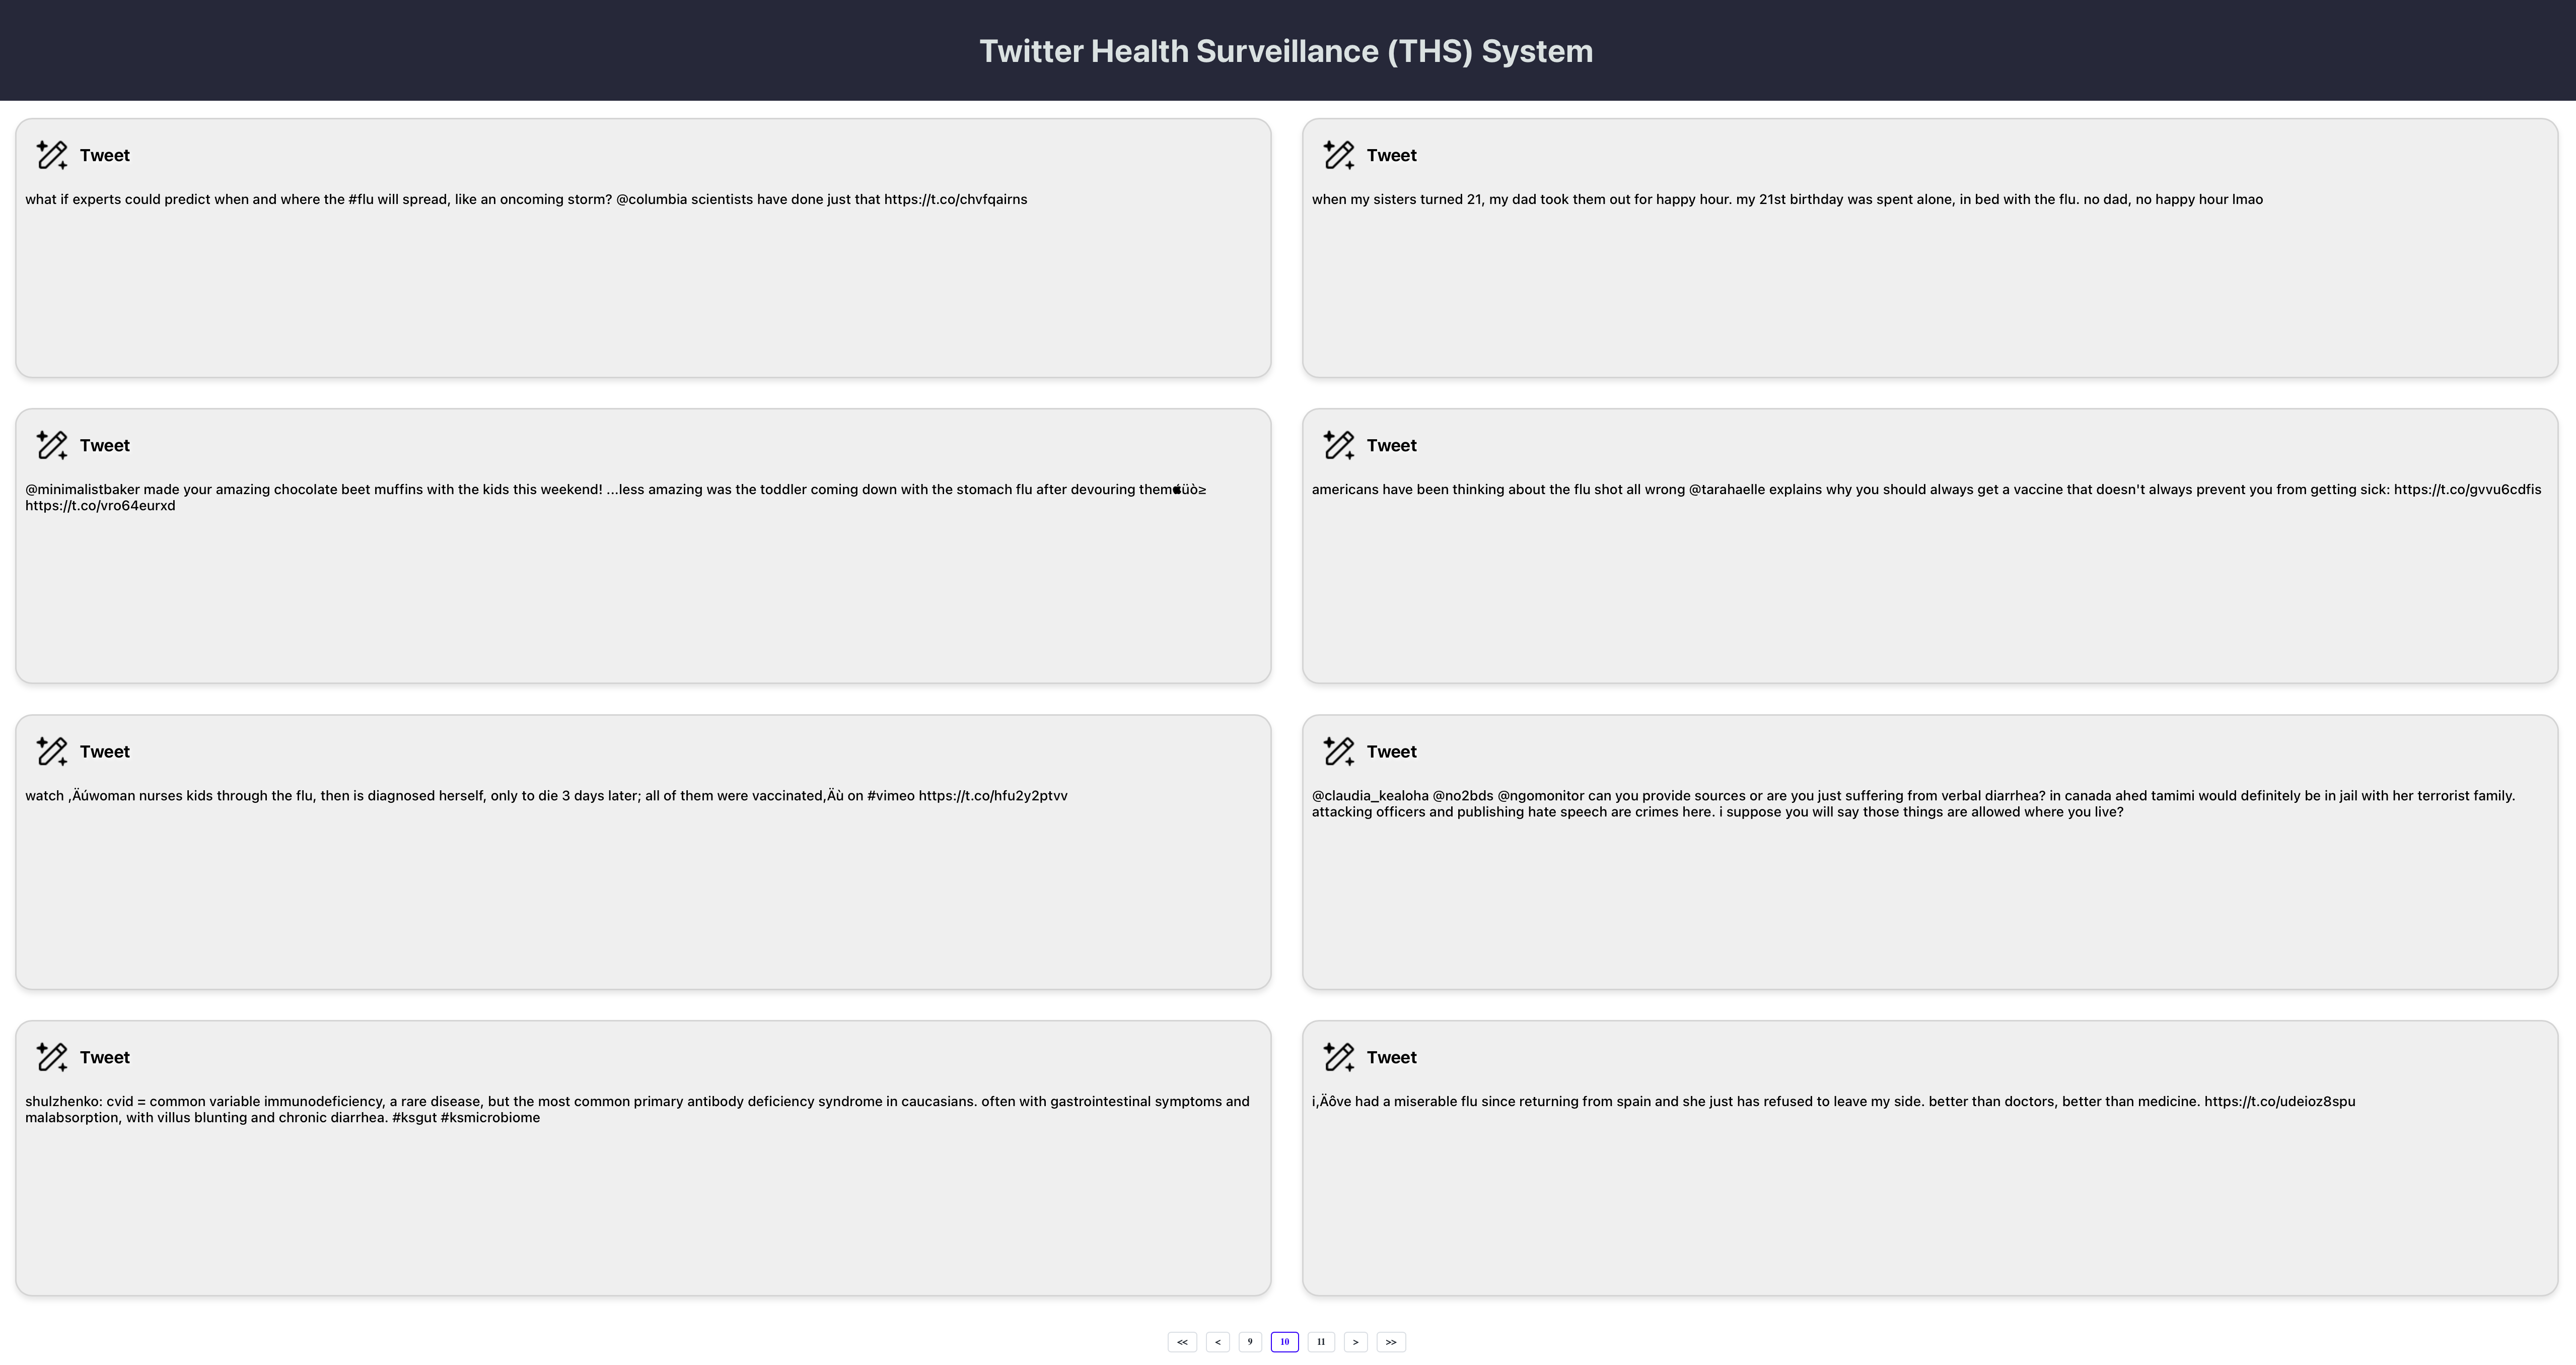
\includegraphics[width=0.67\paperwidth]{images/THS_Frontend_Menu.png}} %specify width
	\end{center}

%\noindent\makebox[\textwidth][l] {%
%	\hspace{-\dimexpr\oddsidemargin+0.375cm} % -\dimexpr\oddsidemargin+0.1\paperwidth -> x * 0.5 - 0.375 (x = width)
%		\frame{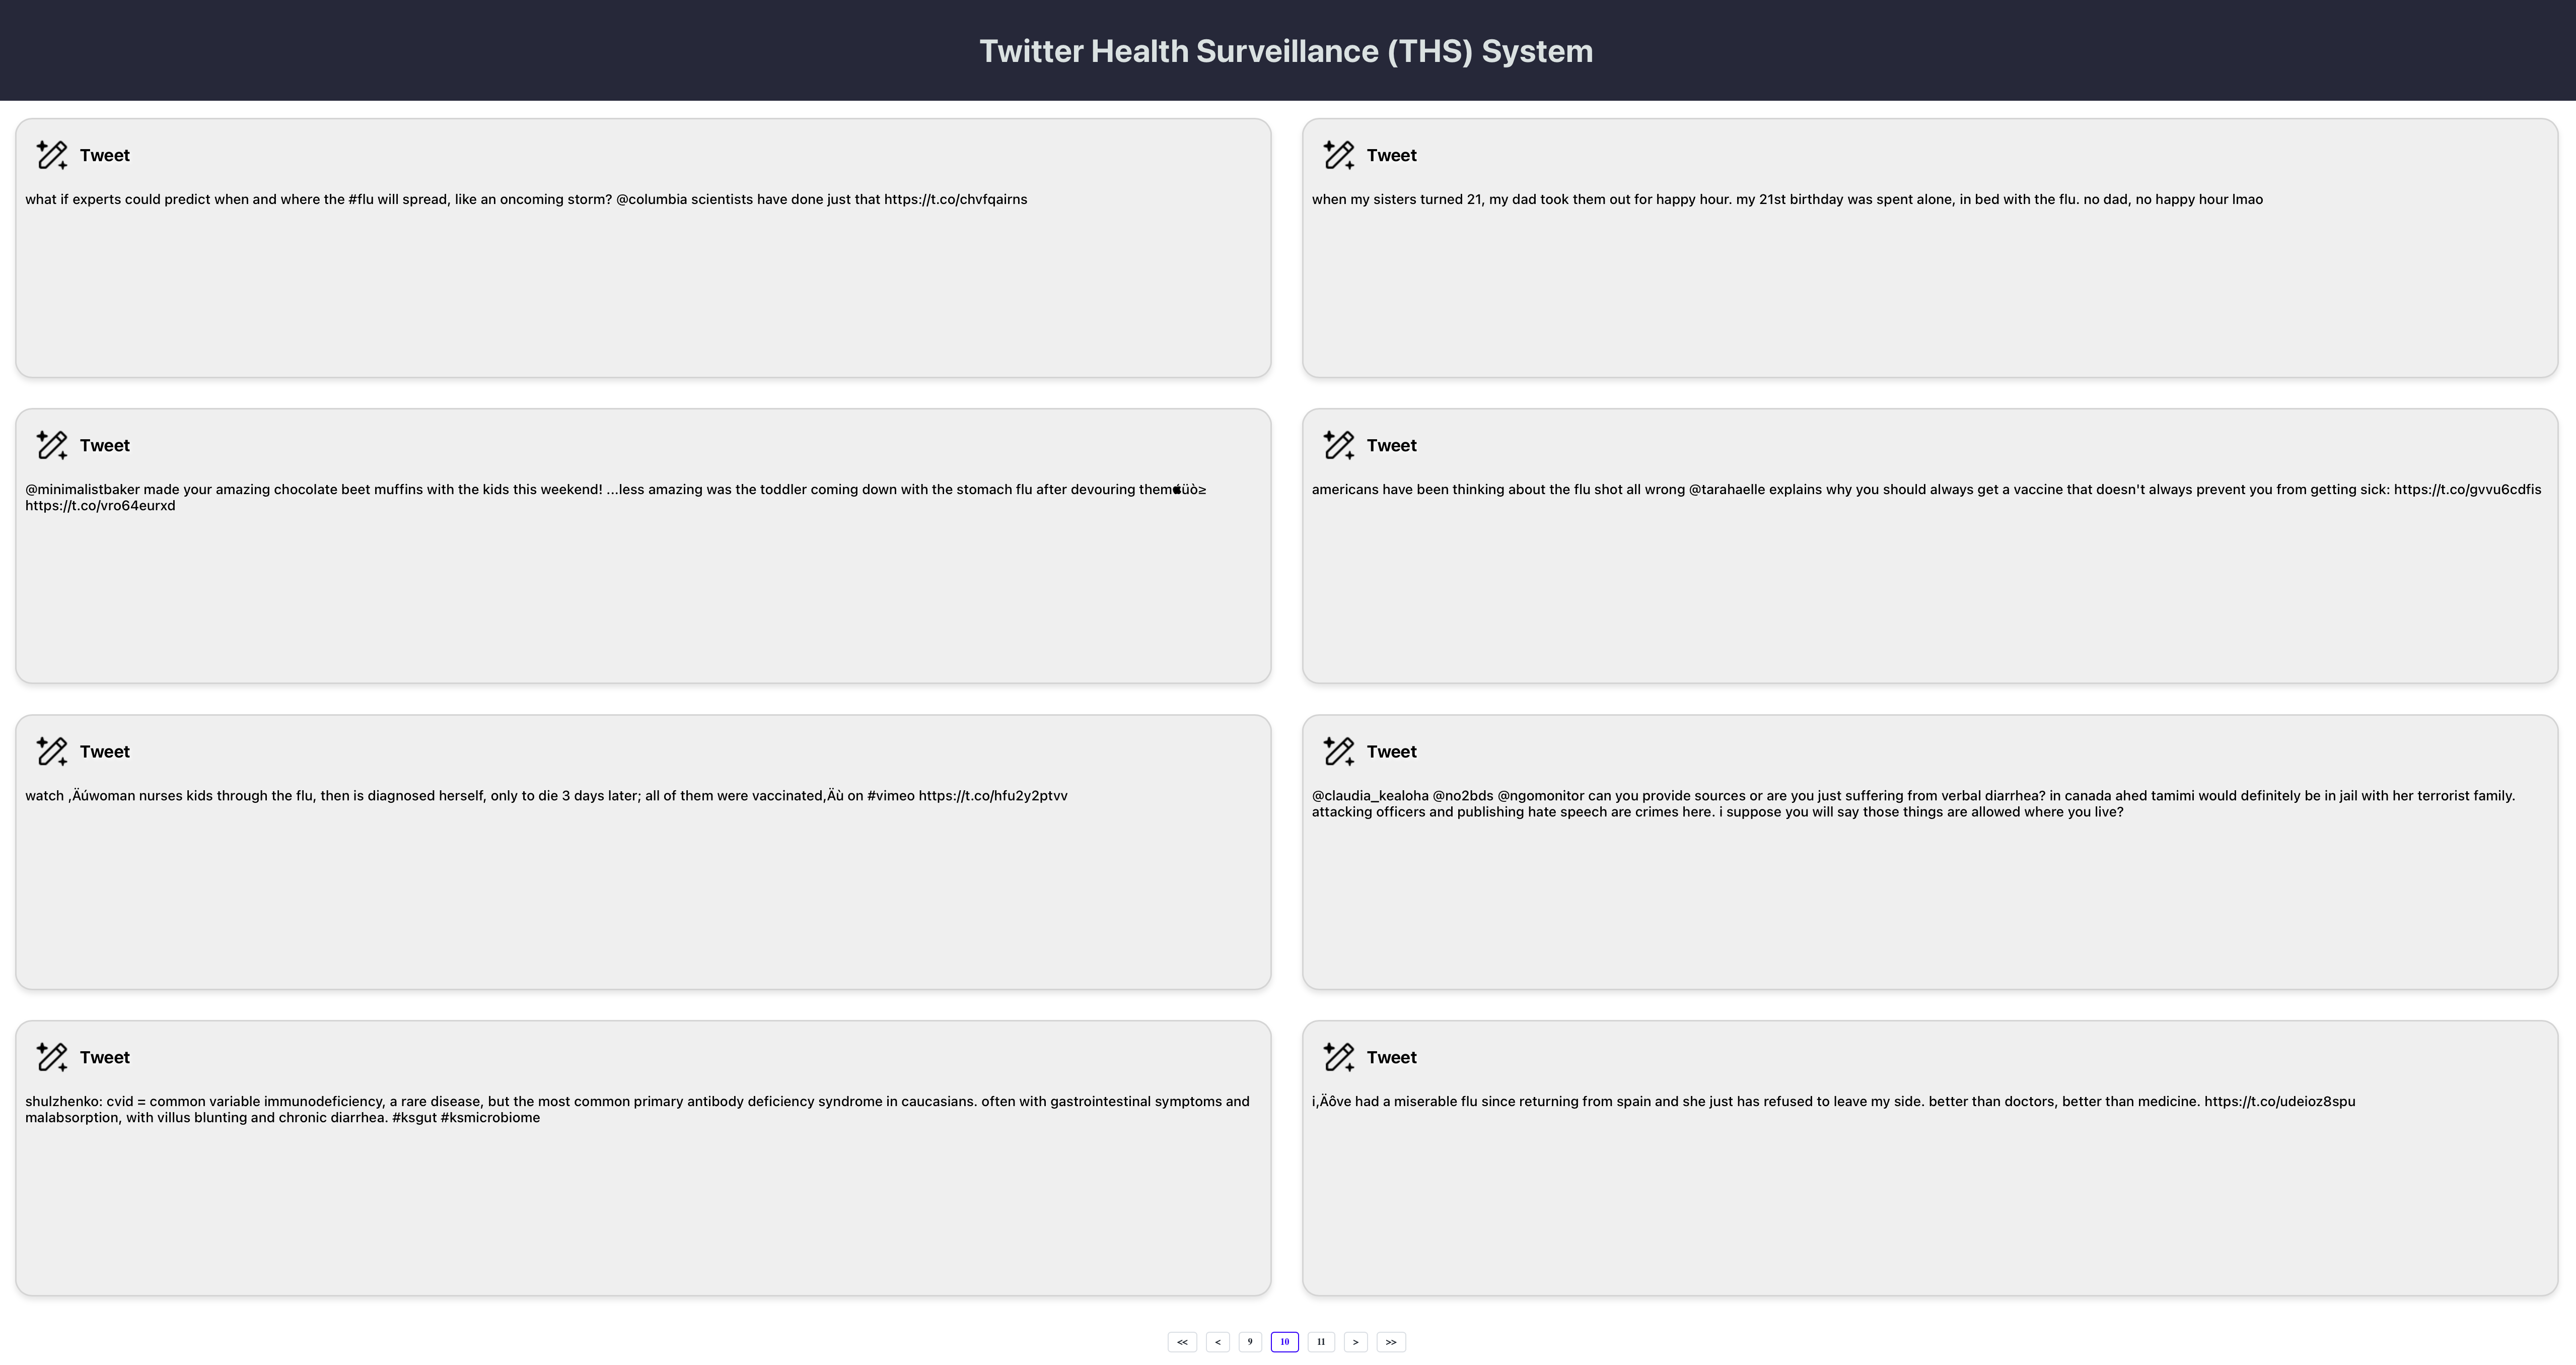
\includegraphics[width=0.70\paperwidth]{images/THS_Frontend_Menu.png}} %specify width
%	}%
	\caption{THS Frontend - Menu} %specify caption
	\label{fig:Menu}
\end{figure}

Figure \ref{fig:frontendmisinformation} presents a case where the models classified the text as health-related and misinformation. The side windows shows the original text, the classifications, and rebuttal. A clearer image of the side screen is shown in Figure \ref{fig:frontendrebuttal}. The top of the side screen shows the text that was classified. Number 1 shows the health classification, and number 2 shows the misinformation classification. Below that is the rebuttal generated by the models. Finally, we include the references of the research used for the rebuttal. 

\begin{figure}[H]
	\begin{center}
		\frame{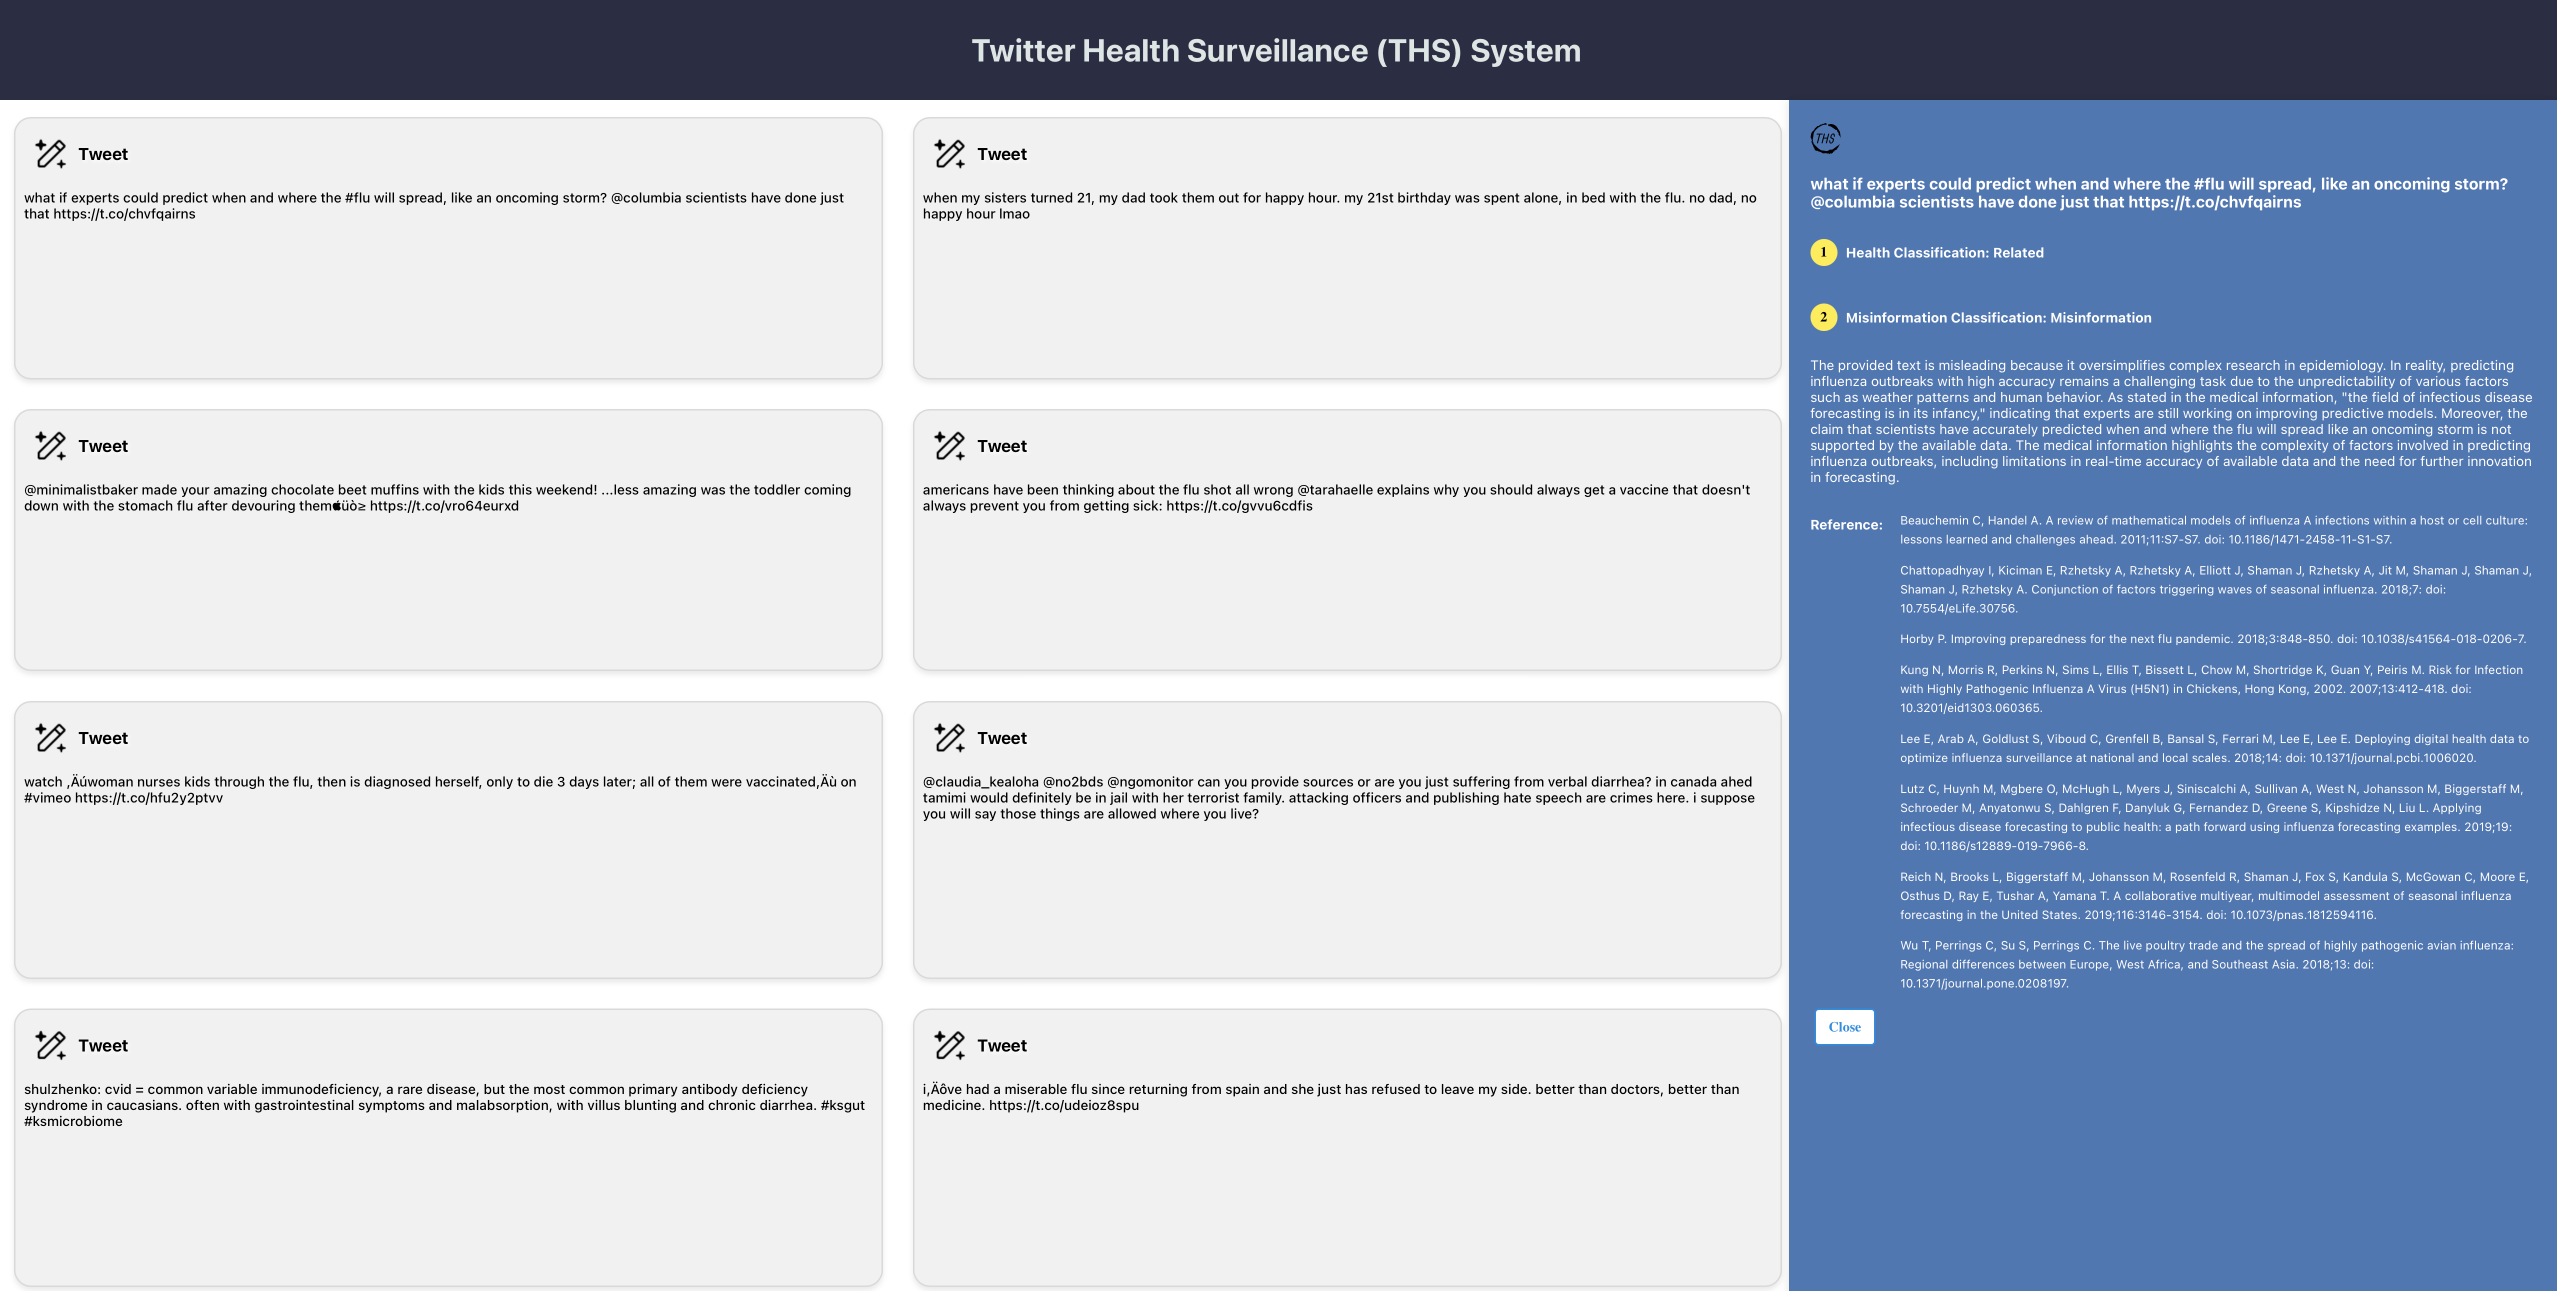
\includegraphics[width=0.67\paperwidth]{images/THS_Misleading.png}} %specify width
	\end{center}

%\noindent\makebox[\textwidth][l] {%
%	\hspace{-\dimexpr\oddsidemargin+0.375in}
%	\frame{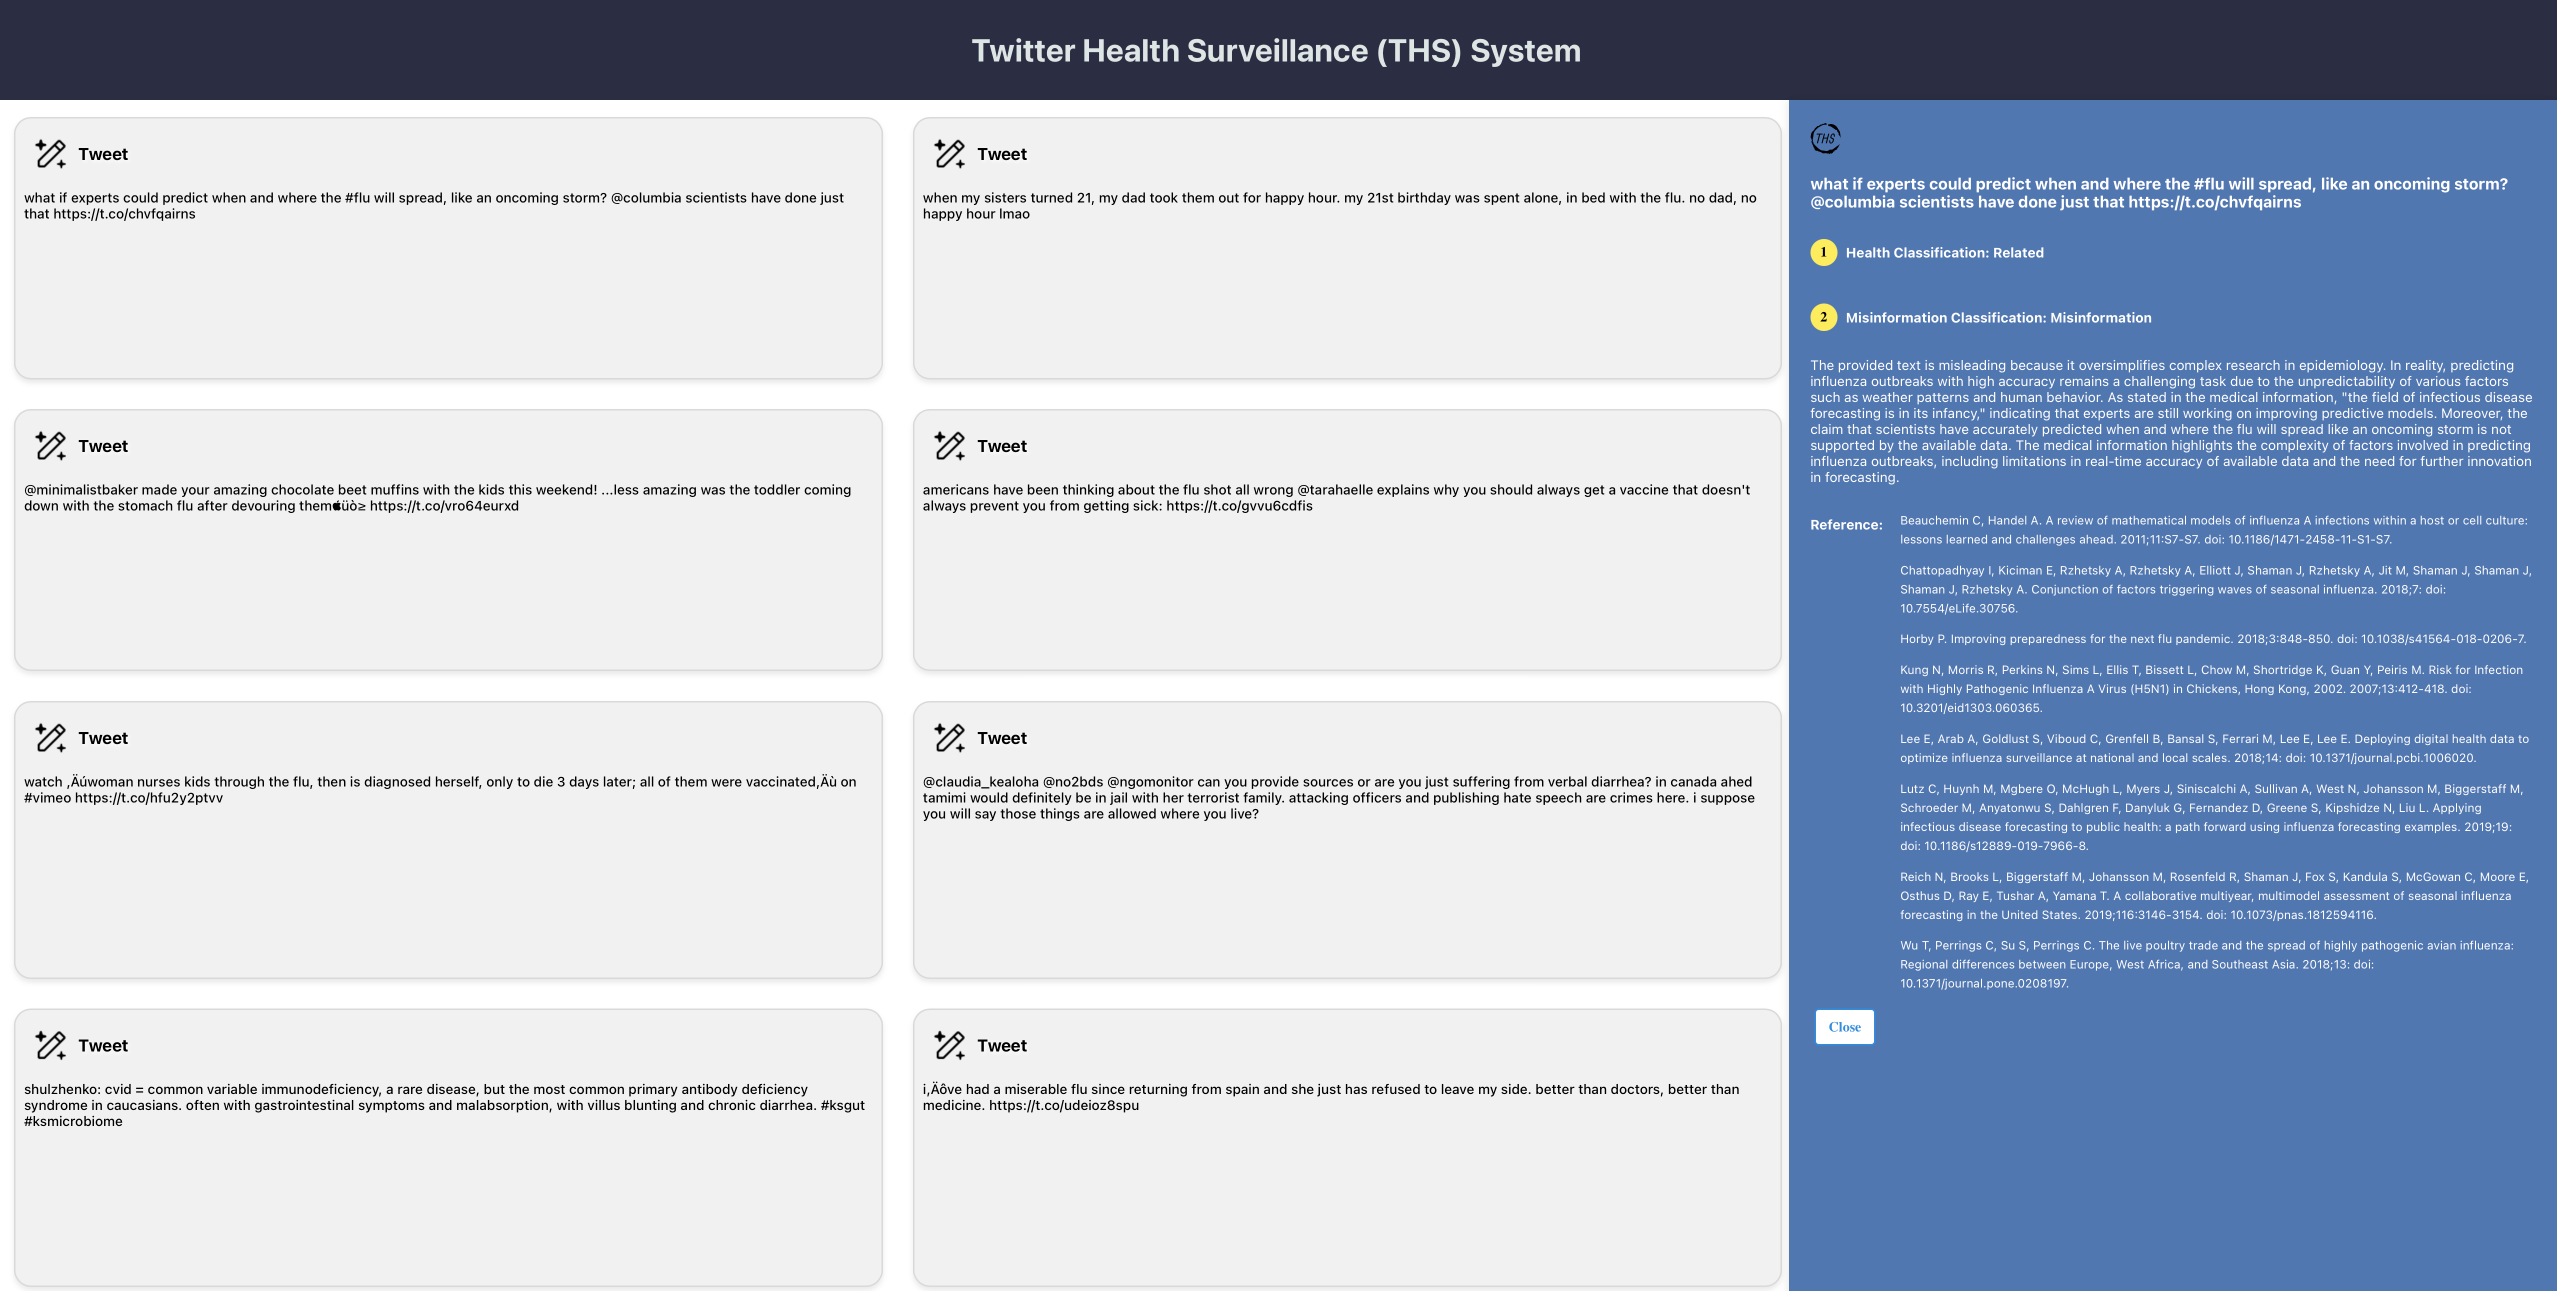
\includegraphics[width=0.70\paperwidth]{images/THS_Misleading.png}} %specify width
%	}%
	\caption{THS Frontend - Misinformation Classification } %specify caption
	\label{fig:frontendmisinformation}
\end{figure}


\begin{figure}[H]
	\begin{center}
		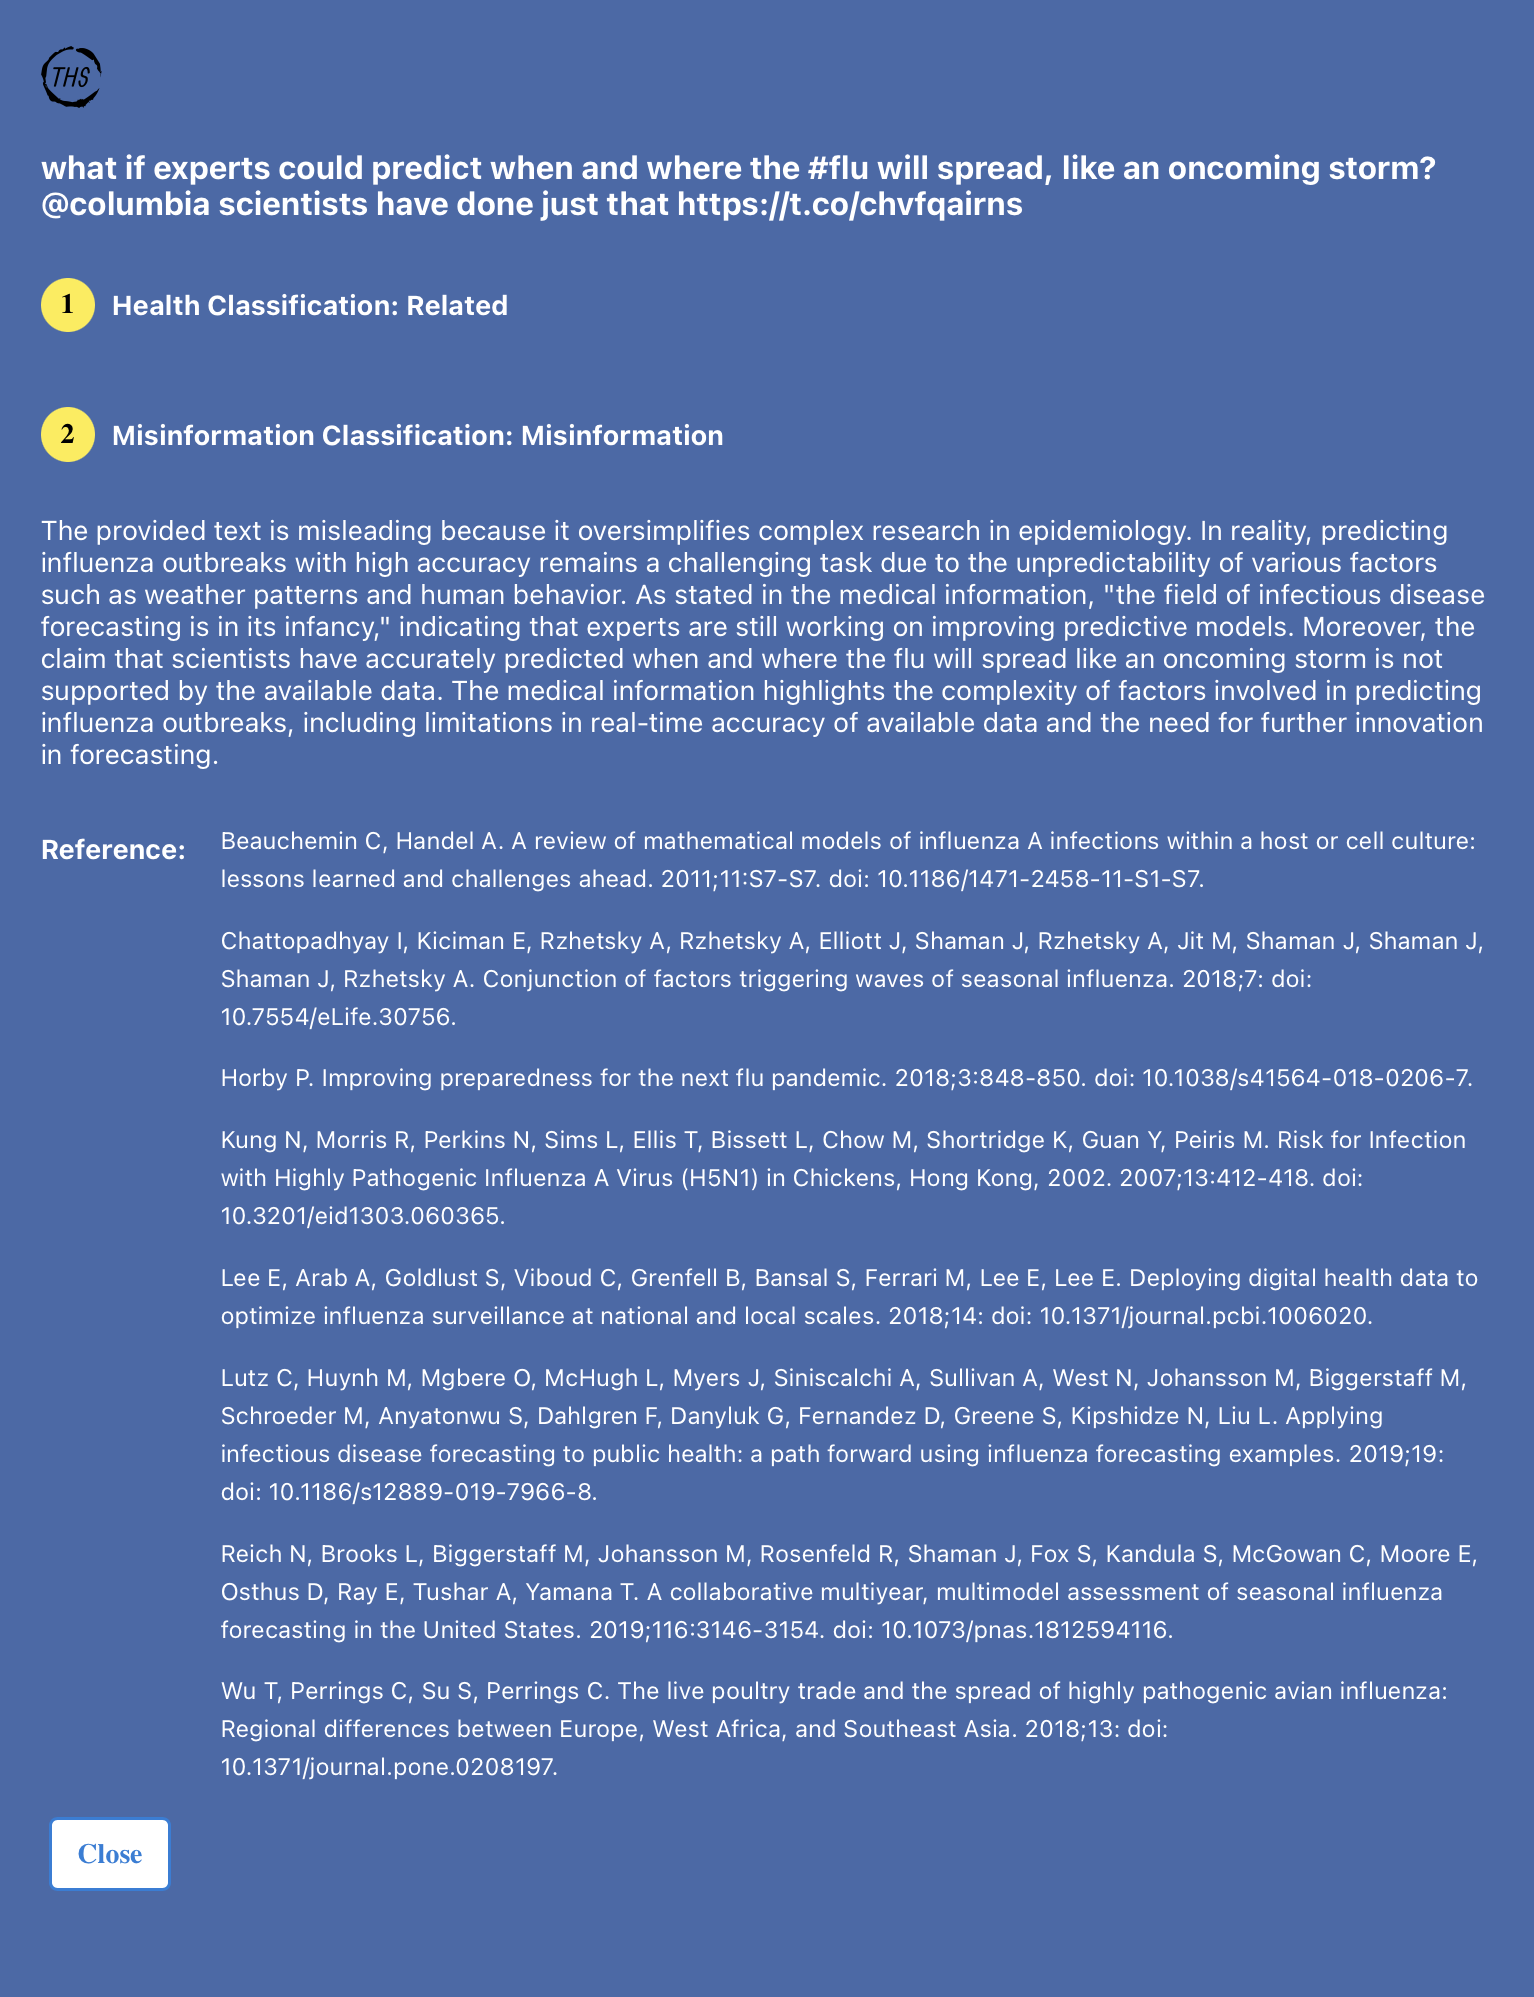
\includegraphics[width=0.75\textwidth]{images/THS_Rebuttal_view.png} %specify width
	\end{center}
	\caption{THS Frontend  - Rebuttal View} %specify caption
	\label{fig:frontendrebuttal}
\end{figure}



